\section{Results}
\label{sec:Results}

In this section, we present whether there is any statistical significance between the results obtained by the two variants of \ApproachName{} (\simhotep{} and \timhotep{}) and the PCG baseline. To do that, we perform the Mann-Whitney U~\cite{mann1947test} setting the confidence limit, $\alpha$, at 0.05, and applying the Bonferroni correction ($\alpha/K$, where K is the number of hypotheses) when multiple hypotheses are tested.  

Unlike parametric tests, the Mann-Whitney U raises the bar for significance, by making no assumptions about underlying data distributions.
Moreover, we used effect size to assess whether the statistical significance has practical significance effect size~\cite{Arcuri2014}. To this end we use the Vargha and Delaney's Â$_{12}$ non-parametric effect size measure, as it is recommended to use a standardised measure rather than a pooled one like the Cohen's $d$ when not all samples are normally distributed~\cite{Arcuri2014}, as in our case. 
The Â$_{12}$ statistic measures the probability that an algorithm $A$ yields greater values for a given performance measure $M$ than another algorithm $B$, based on the following equation: 
\begin{equation}
\hat{A}_{12} = (R_1/m - (m + 1)/2)/n 
\end{equation}
\noindent where $R_1$ is the rank sum of the first data group we are comparing, and $m$ and $n$ are the number of observations in the first and second data sample, respectively. Values between $(0.44, 0.56)$ represent negligible differences, values between $[0.56, 0.64)$ and $(0.36, 0.44]$ represent small differences, values between $[0.64, 0.71)$ and $(0.29, 0:44]$ represent medium differences, and values between $[0.0, 0.29]$ and $[0.71, 1.0]$ represent large differences.

The mean values and standard deviations for $Q_{Duration}$for each \ApproachName{} variants and the baseline are presented in Table~\ref{tab:results}. Both variants (\simhotep{} and \timhotep{}) obtained better results than the baseline (Base). Specifically, $S_{Imhotep}$ yielded the best results, followed by $T_{Imhotep}$ and then baseline.

\begin{table*}[ht!]
\centering
\caption{Mean values and standard deviations for $Q_{Duration}$ for each approach.}
\label{tab:results}
\begin{tabular}{@{}ccccccc@{}}
\toprule
    %& \multicolumn{6}{c}{\ApproachName{} with simulation-based variant ($S_{Imhotep}$)}                                           \\ \cmidrule(l){2-7} 
    & Argos            & Maia              & Orion            & Teuthus           & Vermis            & Overall           \\ \midrule
                                   \rowcolor[HTML]{C0C0C0}
\multicolumn{1}{r}{\cellcolor[HTML]{FFFFFF}{$S_{Imhotep}$}} & 43.92 $\pm$ 9.30 & 43.08 $\pm$ 12.09 & 48.86 $\pm$ 8.69 & 60.78 $\pm$ 7.38  & 69.90 $\pm$ 10.52 & 53.31 $\pm$ 14.26 \\ \midrule
    %& \multicolumn{6}{c}{\ApproachName{} with test-based variant ($T_{Imhotep}$)}                                                 \\ \cmidrule(l){2-7} 
    %& Argos            & Maia              & Orion            & Teuthus           & Vermis            & Overall           \\ \midrule
\multicolumn{1}{r}{$T_{Imhotep}$} & 32.17 $\pm$ 6.94 & 29.52 $\pm$ 9.34  & 31.41 $\pm$ 6.83 & 46.33 $\pm$ 10.54 & 42.50 $\pm$ 12.96 & 36.39 $\pm$ 11.72 \\ \midrule
    %& \multicolumn{6}{c}{PCG Baseline (Base)}                                                                             \\ \cmidrule(l){2-7} 
    %& Argos            & Maia              & Orion            & Teuthus           & Vermis            & Overall           \\ \midrule
\multicolumn{1}{r}{Baseline} & 20.15 $\pm$ 1.86 & 8.43 $\pm$ 1.81   & 32.97 $\pm$ 0.85 & 19.53 $\pm$ 1.88  & 25.48 $\pm$ 3.31  & 21.31 $\pm$ 8.32  \\ \bottomrule
\end{tabular}
\end{table*}

Figure~\ref{fig:results} shows the results of the evaluation execution of our approach when using the two objective functions (simulation-Based and test-Based) from \ApproachName{} and the Baseline. The executions are grouped by each host (boss of \CaseStudy{}) that has been used in our experiment (Argos, Maia, Orion, Teuthus, and Vermis). The last column, with shaded background, shows the average of all the hosts for each objective function and the baseline. 

Each boxplot is generated from the results of each host obtained from transplantation \ApproachName{} or generation (baseline). Each boxplot represents 645 values of a specific host-organ transplantation (\ApproachName{}) or 645 generations from a specific host (baseline). Each value in the boxplot is the mean value (between the 30 independent runs) of the quality indicator ($Q_{Duration}$) for one of the transplants (\ApproachName{}) or generations (baseline).

\subsection{Research Question 1: \simhotep{} vs Baseline}

\begin{table}[ht!]
    \centering
    \caption{Mann-Withney U pair-wise test results / Vargha-Delaney Â$_{12}$ effect sizes obtained comparing \simhotep{} and the PCG Baseline. Â$_{12}$: Large -- L.}
    \label{tab:results_rq1}
    \begin{tabular}{@{}rc@{}}
    \toprule
    Boss    & $p-Value$ / Â$_{12}$           \\ \midrule 
    Argos   & $3.25x10^{-23}$  / 0.99 (L)    \\
    Maia    & $3.25x10^{-23}$  /  1.0 (L)    \\
    Orion   & $4.01x10^{-23}$  / 0.98 (L)    \\
    Teuthus & $3.25x10^{-23}$  /  1.0 (L)    \\
    Vermis  & $3.25x10^{-23}$  /  1.0 (L)    \\
    Overall & $1.41x10^{-107}$ / 0.98 (L)    \\
    \bottomrule
    \end{tabular}
    \end{table}

The variants obtained an average value of 44.85\% in $Q_{Duration}$, with \simhotep{} being the variant that obtained the best results overall (53.31\% in $Q_{Duration}$). \timhotep obtained 36.39\% in the overall $Q_{Duration}$, which also outperformed the baseline. The baseline obtained the worst $Q_{Duration}$. All in all, the results reveal that leveraging simulations as objective function pays off in the context of PCT, yielding 1.5x better results than the test-based variant and 2.5x better results than baseline.

\subsection{Research Question 2: \simhotep{} vs \timhotep{}}

\begin{table}[ht!]
    \centering
    \caption{Mann-Withney U pair-wise test results / Vargha-Delaney Â$_{12}$ effect sizes obtained comparing \simhotep{} and \timhotep{}. Â$_{12}$: Large -- L.}
    \label{tab:results_rq2}
    \begin{tabular}{@{}rc@{}}
    \toprule
    Boss    & $p-Value$ / Â$_{12}$           \\ \midrule 
    Argos   & $1.28x10^{-18}$ / 0.85 (L)     \\
    Maia    & $6.64x10^{-18}$ / 0.85 (L)     \\
    Orion   & $4.95x10^{-22}$ / 0.95 (L)     \\
    Teuthus & $3.60x10^{-18}$ / 0.87 (L)     \\
    Vermis  & $8.86x10^{-23}$ / 0.95 (L)     \\
    Overall & $6.58x10^{-93}$ / 0.82 (L)     \\
    \bottomrule
    \end{tabular}
    \end{table}

% To properly compare the approaches, all of the data resulting from the empirical analysis was analyzed using statistical methods following the guidelines by Arcuri \etal~\cite{Arcuri2014}.

% The analysis that we must follow depends on the properties of the data. Since our data does not follow a normal distribution in general, our analysis requires the use of non-parametric techniques. There are several tests for analyzing this kind of data; however, the Quade test has shown that it is more powerful than the others when working with real data~\cite{Garcia2010}. In addition, according to Conover~\cite{Conover1999}, the Quade test has shown better results than the others when the number of algorithms is low (no more than four or five algorithms).

The obtained $p-values$ for $Q_{Duration}$ are less than $2.2x10^{-16}$. Since the $p-Values$ are smaller than 0.05, we can state that there are differences among the algorithms for the quality indicator of $Q_{Duration}$.

% \begin{table}[H]
% \centering
% \caption{Holm's post hoc $p-Values$ for each pair-wise comparison.}
% \label{tab:postHoc}
% \begin{tabular}{@{}rcc@{}}
% \toprule
%             \simhotep{} vs   & $p-Values$    & Â$_{12}$   \\ \midrule
%             Baseline         & $<2x10^{-16}$ & 0.0121531  \\
%             \timhotep{}      & $<2x10^{-16}$ & 0.1712710  \\
%             %$T_{Imhotep}$ vs Base  & $<2x10^{-16}$  \\ 
%             \bottomrule
% \end{tabular}
% \end{table}

%However, with the Quade test, we cannot know which of the algorithms gives the best performance. In this case, the performance of each algorithm should be individually compared against all of the other alternatives. In order to do this, we perform an additional post hoc analysis. This kind of analysis performs a pair-wise comparison among the results of each algorithm, determining whether statistically significant differences exist among the results of a specific pair of algorithms.
Table~\ref{tab:postHoc} shows the $p-Values$ of the Holm's post hoc analysis for each pair-wise comparison and quality indicator. All of the $p-Values$ obtained in $Q_{Duration}$ were smaller than their corresponding significance threshold value ($0.05$), indicating that the differences in solution quality between the two variants and the baseline are significant.

\textbf{RQ$_2$ answer. }
Since the Holm's post hoc $p-values$ for $Q_{Duration}$ (shown in Table~\ref{tab:postHoc}) are smaller than $0.05$, we can state that there are significant differences between the variants and the baseline.

%\subsection{Research Question 3: Magnitude}

When comparing algorithms with a large enough number of runs, statistically significant differences can be obtained even if they are so small as to be of no practical value~\cite{Arcuri2014}. Thus, it is important to assess if an algorithm is statistically better than another and to assess the magnitude of the improvement. Effect size measures are needed to analyze this.

% \begin{table}[H]
% \centering
% \caption{Effect size measures for comparing each pair of algorithms in \CaseStudy{}.}
% \label{tab:effectSize}
% \begin{tabular}{@{}rc@{}}
% \toprule
% $S_{Imhotep}$ vs      & Â$_{12}$          \\ \cmidrule(l){2-2} 
%                %& $Q_{Duration}$    \\ \midrule
% Baseline  & 0.0121531         \\
% $T_{Imhotep}$ & 0.1712710         \\
% % & 0.1411910         \\ \midrule
% %                & Cliff's Delta     \\ \cmidrule(l){2-2} 
% %                & $Q_{Duration}$    \\ \midrule
% %                $S_{Imhotep}$ vs Base  & 0.9756914 (large) \\
% % $S_{Imhotep}$ vs $T_{Imhotep}$ & 0.6574437 (large) \\
% % $T_{Imhotep}$ vs Base  & 0.7175939 (large) \\ 
% \bottomrule
% \end{tabular}
% \end{table}

For a non-parametric effect size measure, we use Vargha and Delaney's Â$_{12}$~\cite{Vargha2000,Grissom2005}. Â$_{12}$ measures the probability that running one algorithm yields higher values than running another algorithm. If the two algorithms are equivalent, then Â$_{12}$ will be 0.5.

Table~\ref{} shows the values of the effect size statistics between pair-wise comparisons of algorithms in \CaseStudy{}. Specifically, the upper part of the table shows the Â$_{12}$ values, whereas the lower part of the table shows Cliff's Delta~\cite{Cliff1996} values for $Q_{Duration}$. From the results, we can determine that the performance results obtained by \ApproachName{} with the simulation-based variant, \ApproachName{} with the test-based variant, and the PCG baseline are significant in $Q_{Duration}$. The magnitude of improvement using \ApproachName{} instead of the baseline can be interpreted as being large based on the magnitude scales~\cite{Romano2006} of the Cliff's Delta values. Hence, \ApproachName{} has an actual impact on performance. The highest differences between \ApproachName{} and the baseline are obtained when the simulation-based variant is used, obtaining better results in $Q_{Duration}$ for 97\% of the runs.

%\textbf{RQ$_3$ answer. }
We can draw conclusions about how much the quality of the solution is influenced by each variant of \ApproachName{} compared to baseline from the results of Table~\ref{}. The results reveal that the magnitude of improvement in $Q_{Duration}$ using any variant is large compared to the baseline according to the magnitude scales~\cite{Romano2006} of the Cliff's Delta values.


\begin{figure*}[ht!]
    \centering
    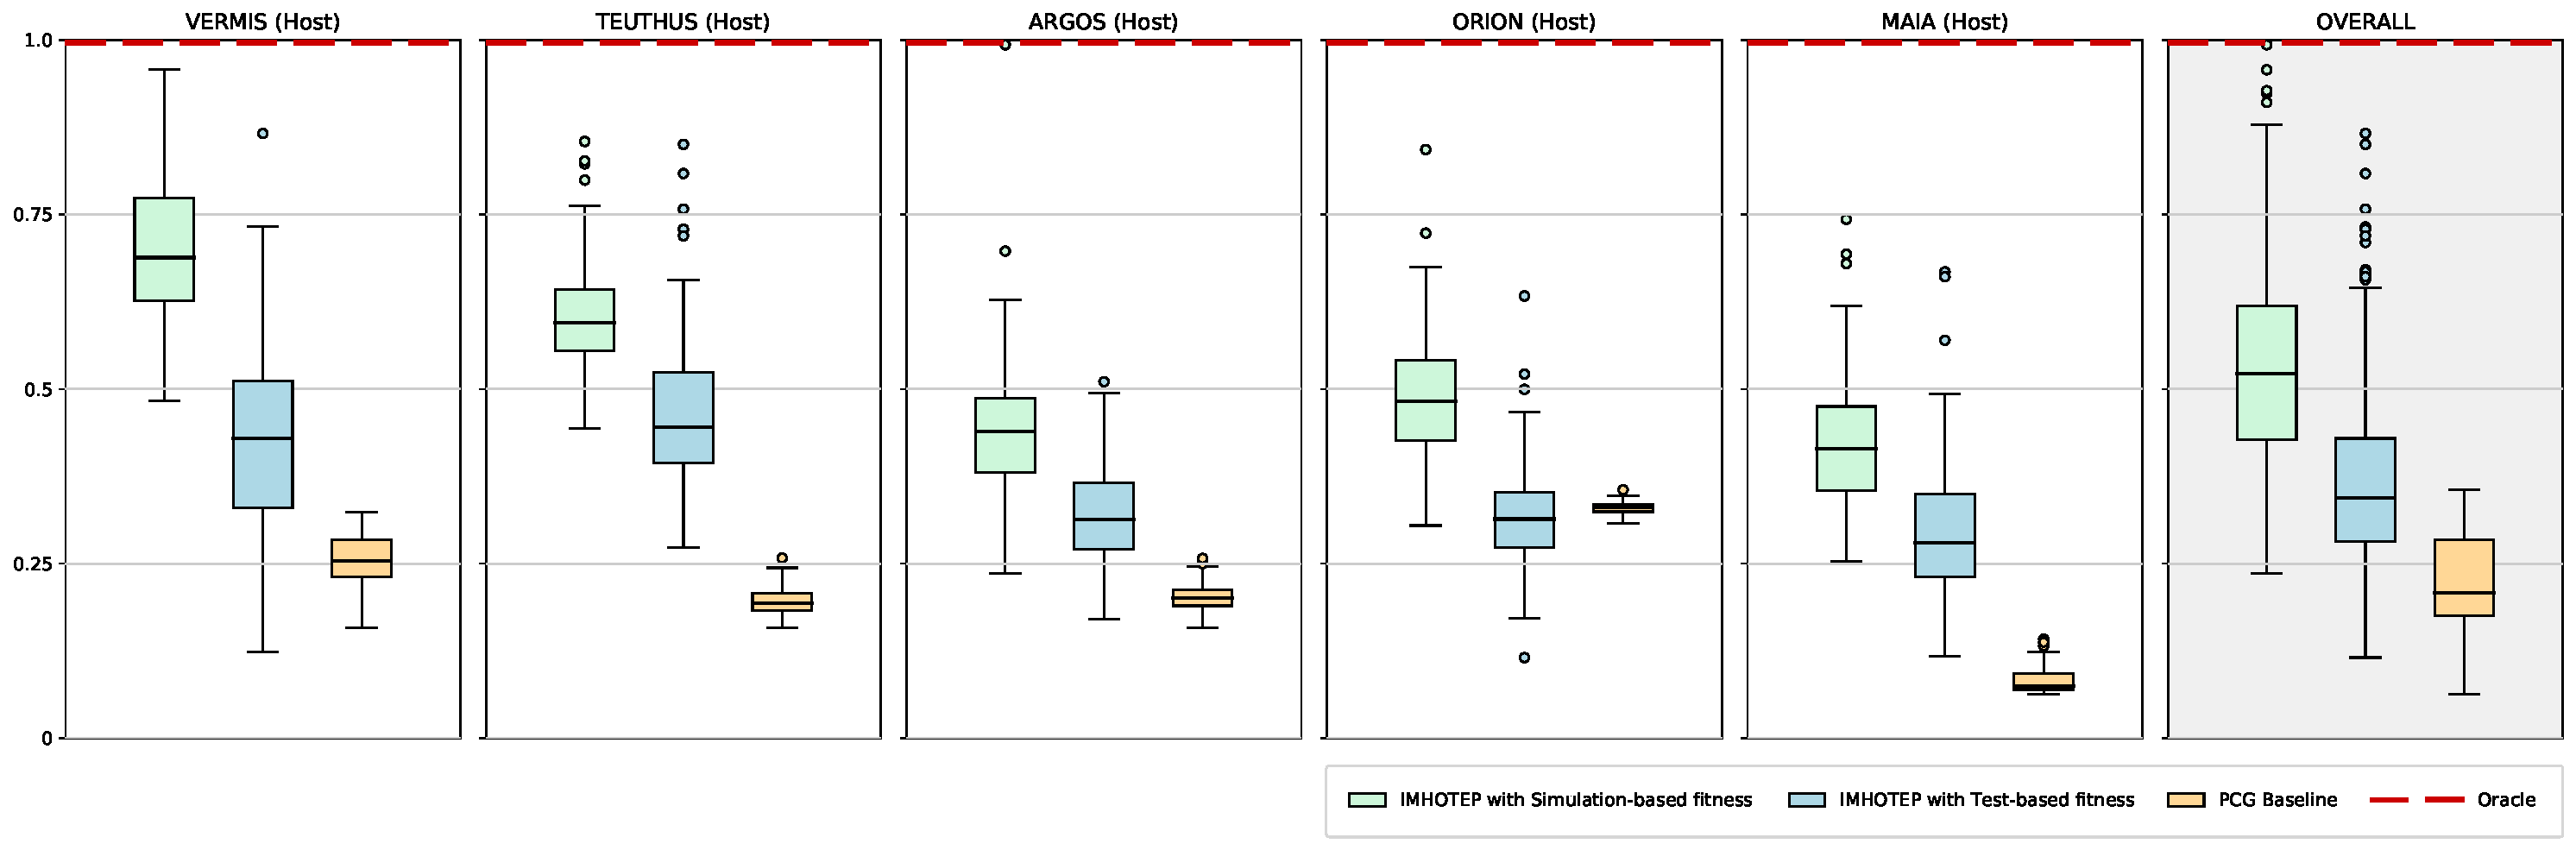
\includegraphics[width=\textwidth]{Figures/Imhotep_with_legend_and_oracle_average-v4.pdf}
    \caption{Results of our \ApproachName{} approaches (simulation-based and test-based) and the baseline for the quality measurement ($Q_{Duration}$).}
    \label{fig:results}
\end{figure*}